\documentclass{article}

\usepackage[dvipdfm]{graphicx}
%\usepackage{amsmath}
\usepackage{amssymb}
\usepackage{color}
\usepackage{wasysym}
\usepackage{rotating}
\usepackage{framed}
\usepackage{pict2e}
\usepackage{tikz}
\usetikzlibrary{decorations.pathreplacing,arrows}
\usepackage{pstricks,pst-node,pst-coil,pst-plot,pst-text}
\usepackage{pstricks-add}


\pagestyle{empty}
\setcounter{page}{1}

\graphicspath{{FiguresNoLabels/}}


\begin{document}

\setlength{\unitlength}{1mm}



%\begin{picture}(100,100)
%
%\put(0,0){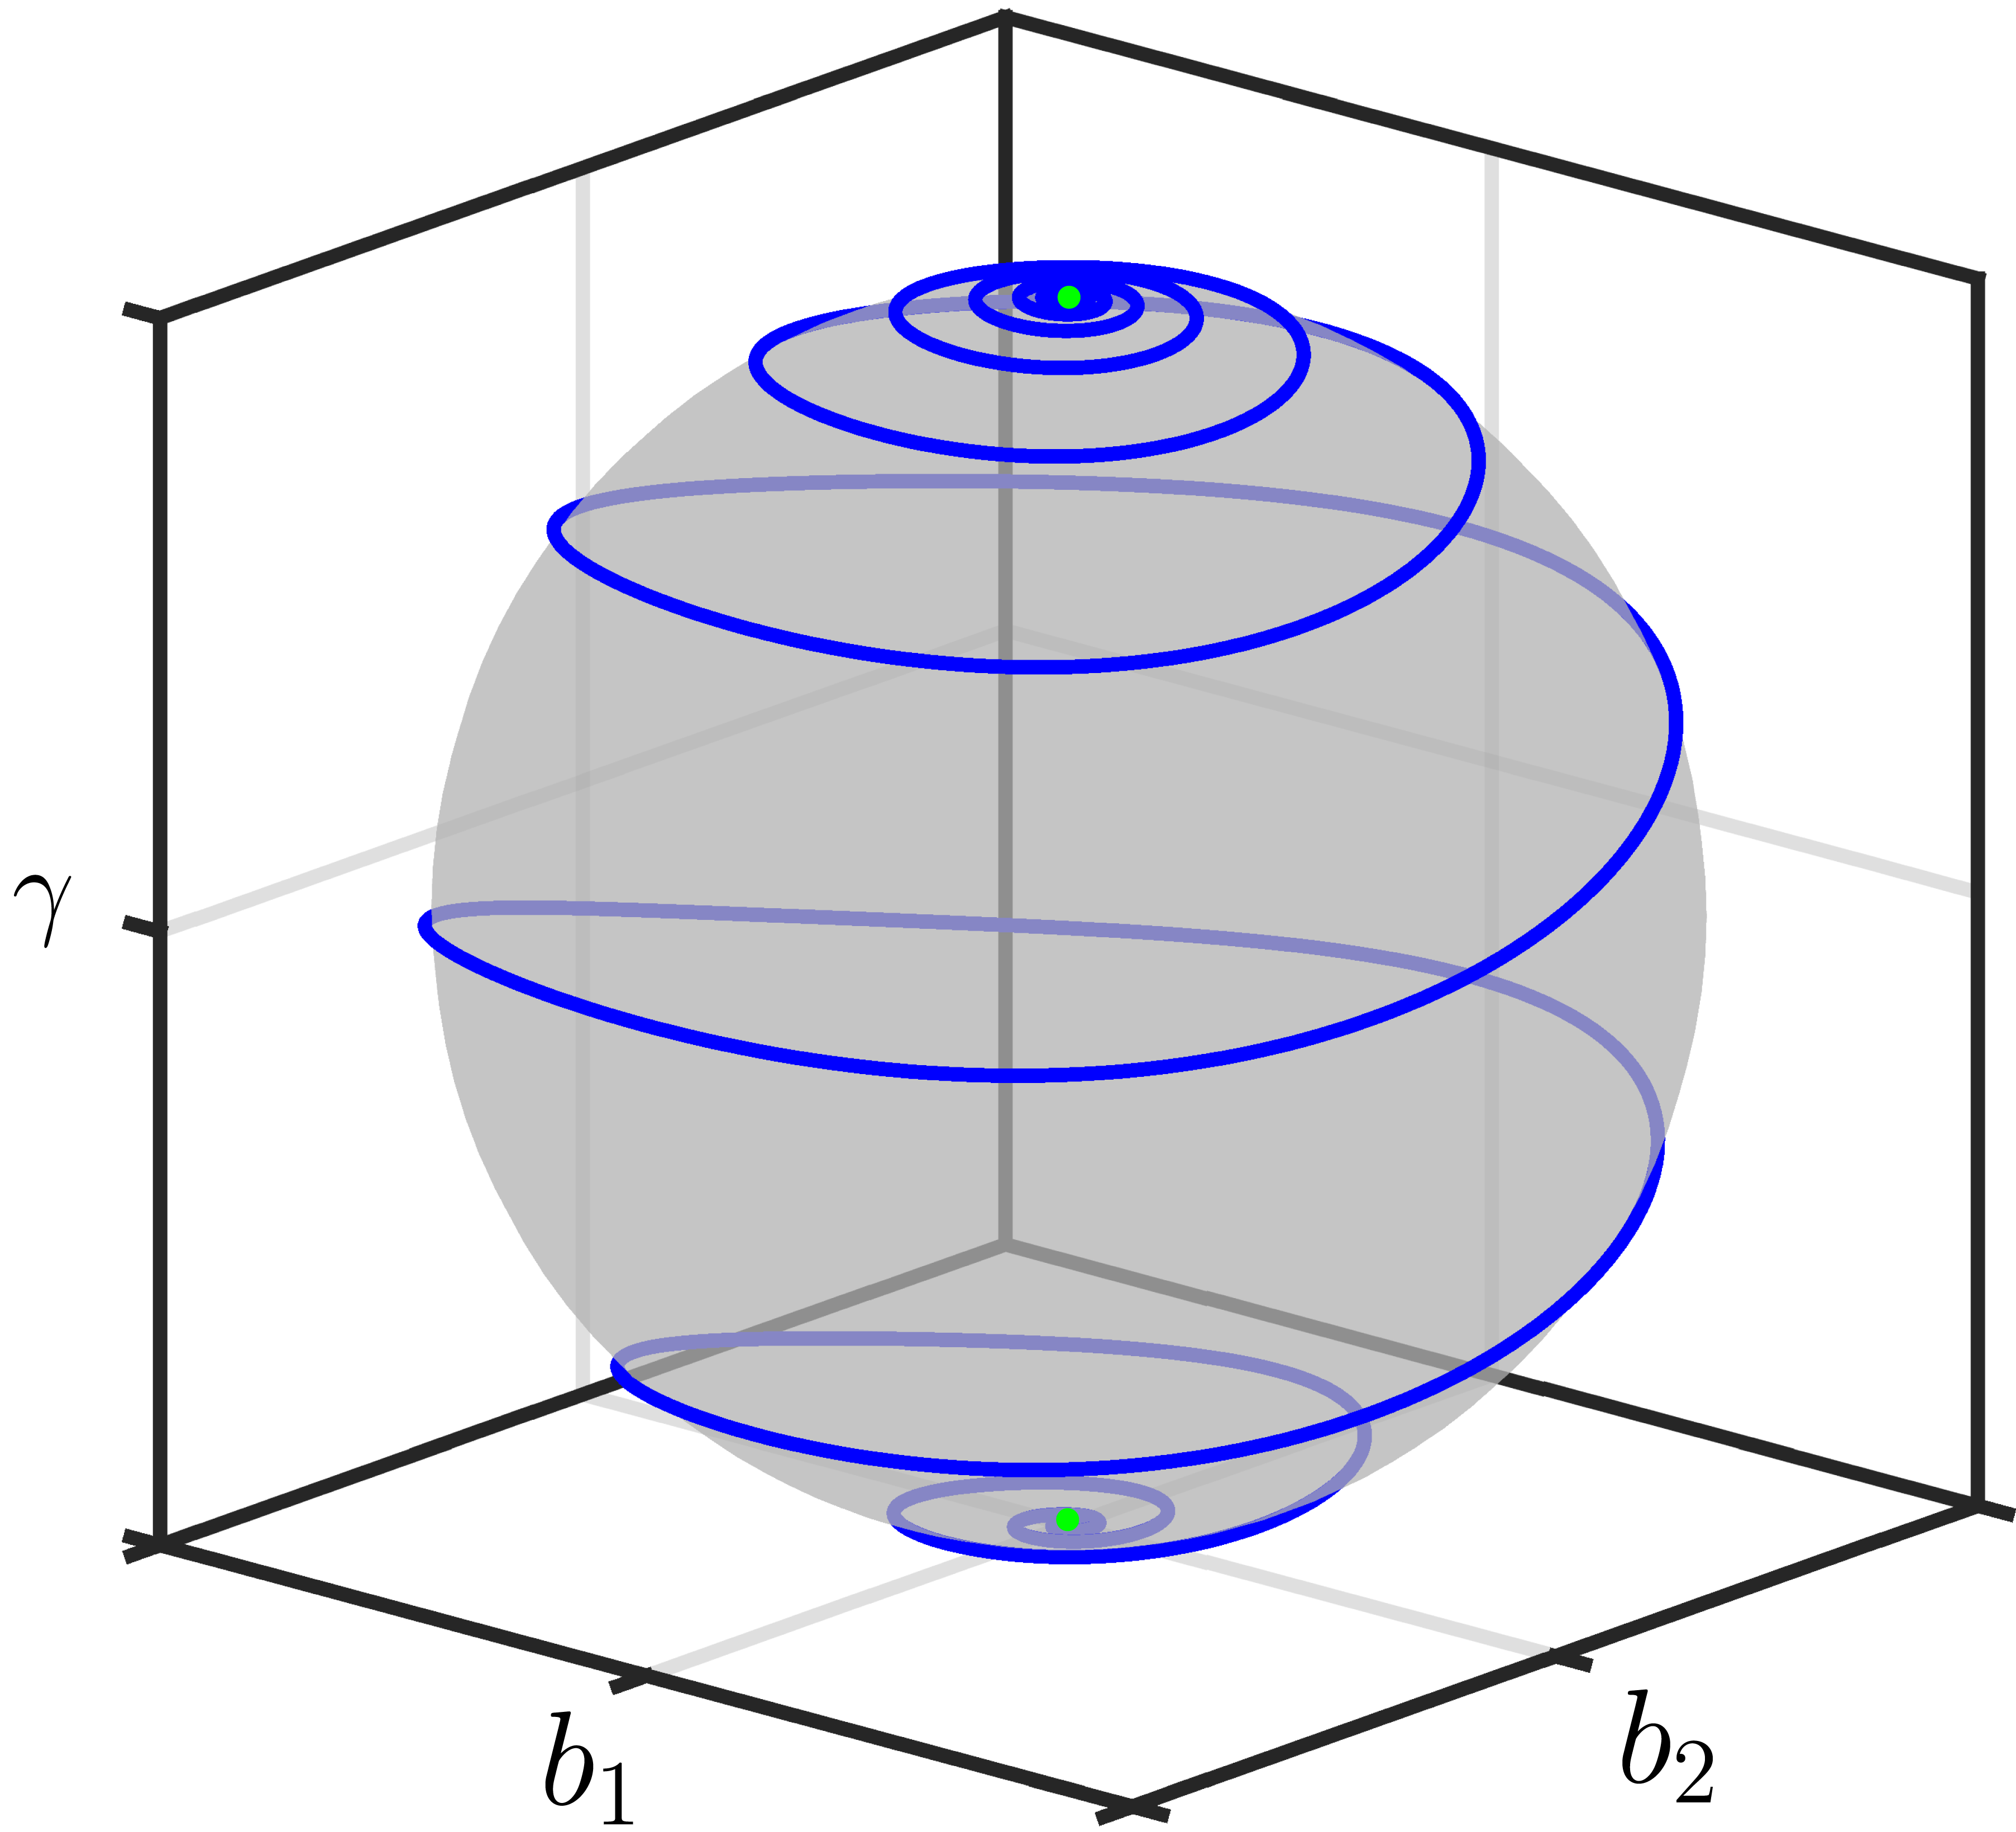
\includegraphics[width=8.6cm]{HTML_BlochSphereNormal.eps}}
%\put(19,1){\LARGE $b_{1}$}
%\put(68,2){\LARGE $b_{2}$}
%\put(-5,41){\LARGE $\gamma$}
%
%
%\end{picture}
%
%\newpage
%
%\begin{picture}(100,100)
%
%\put(0,0){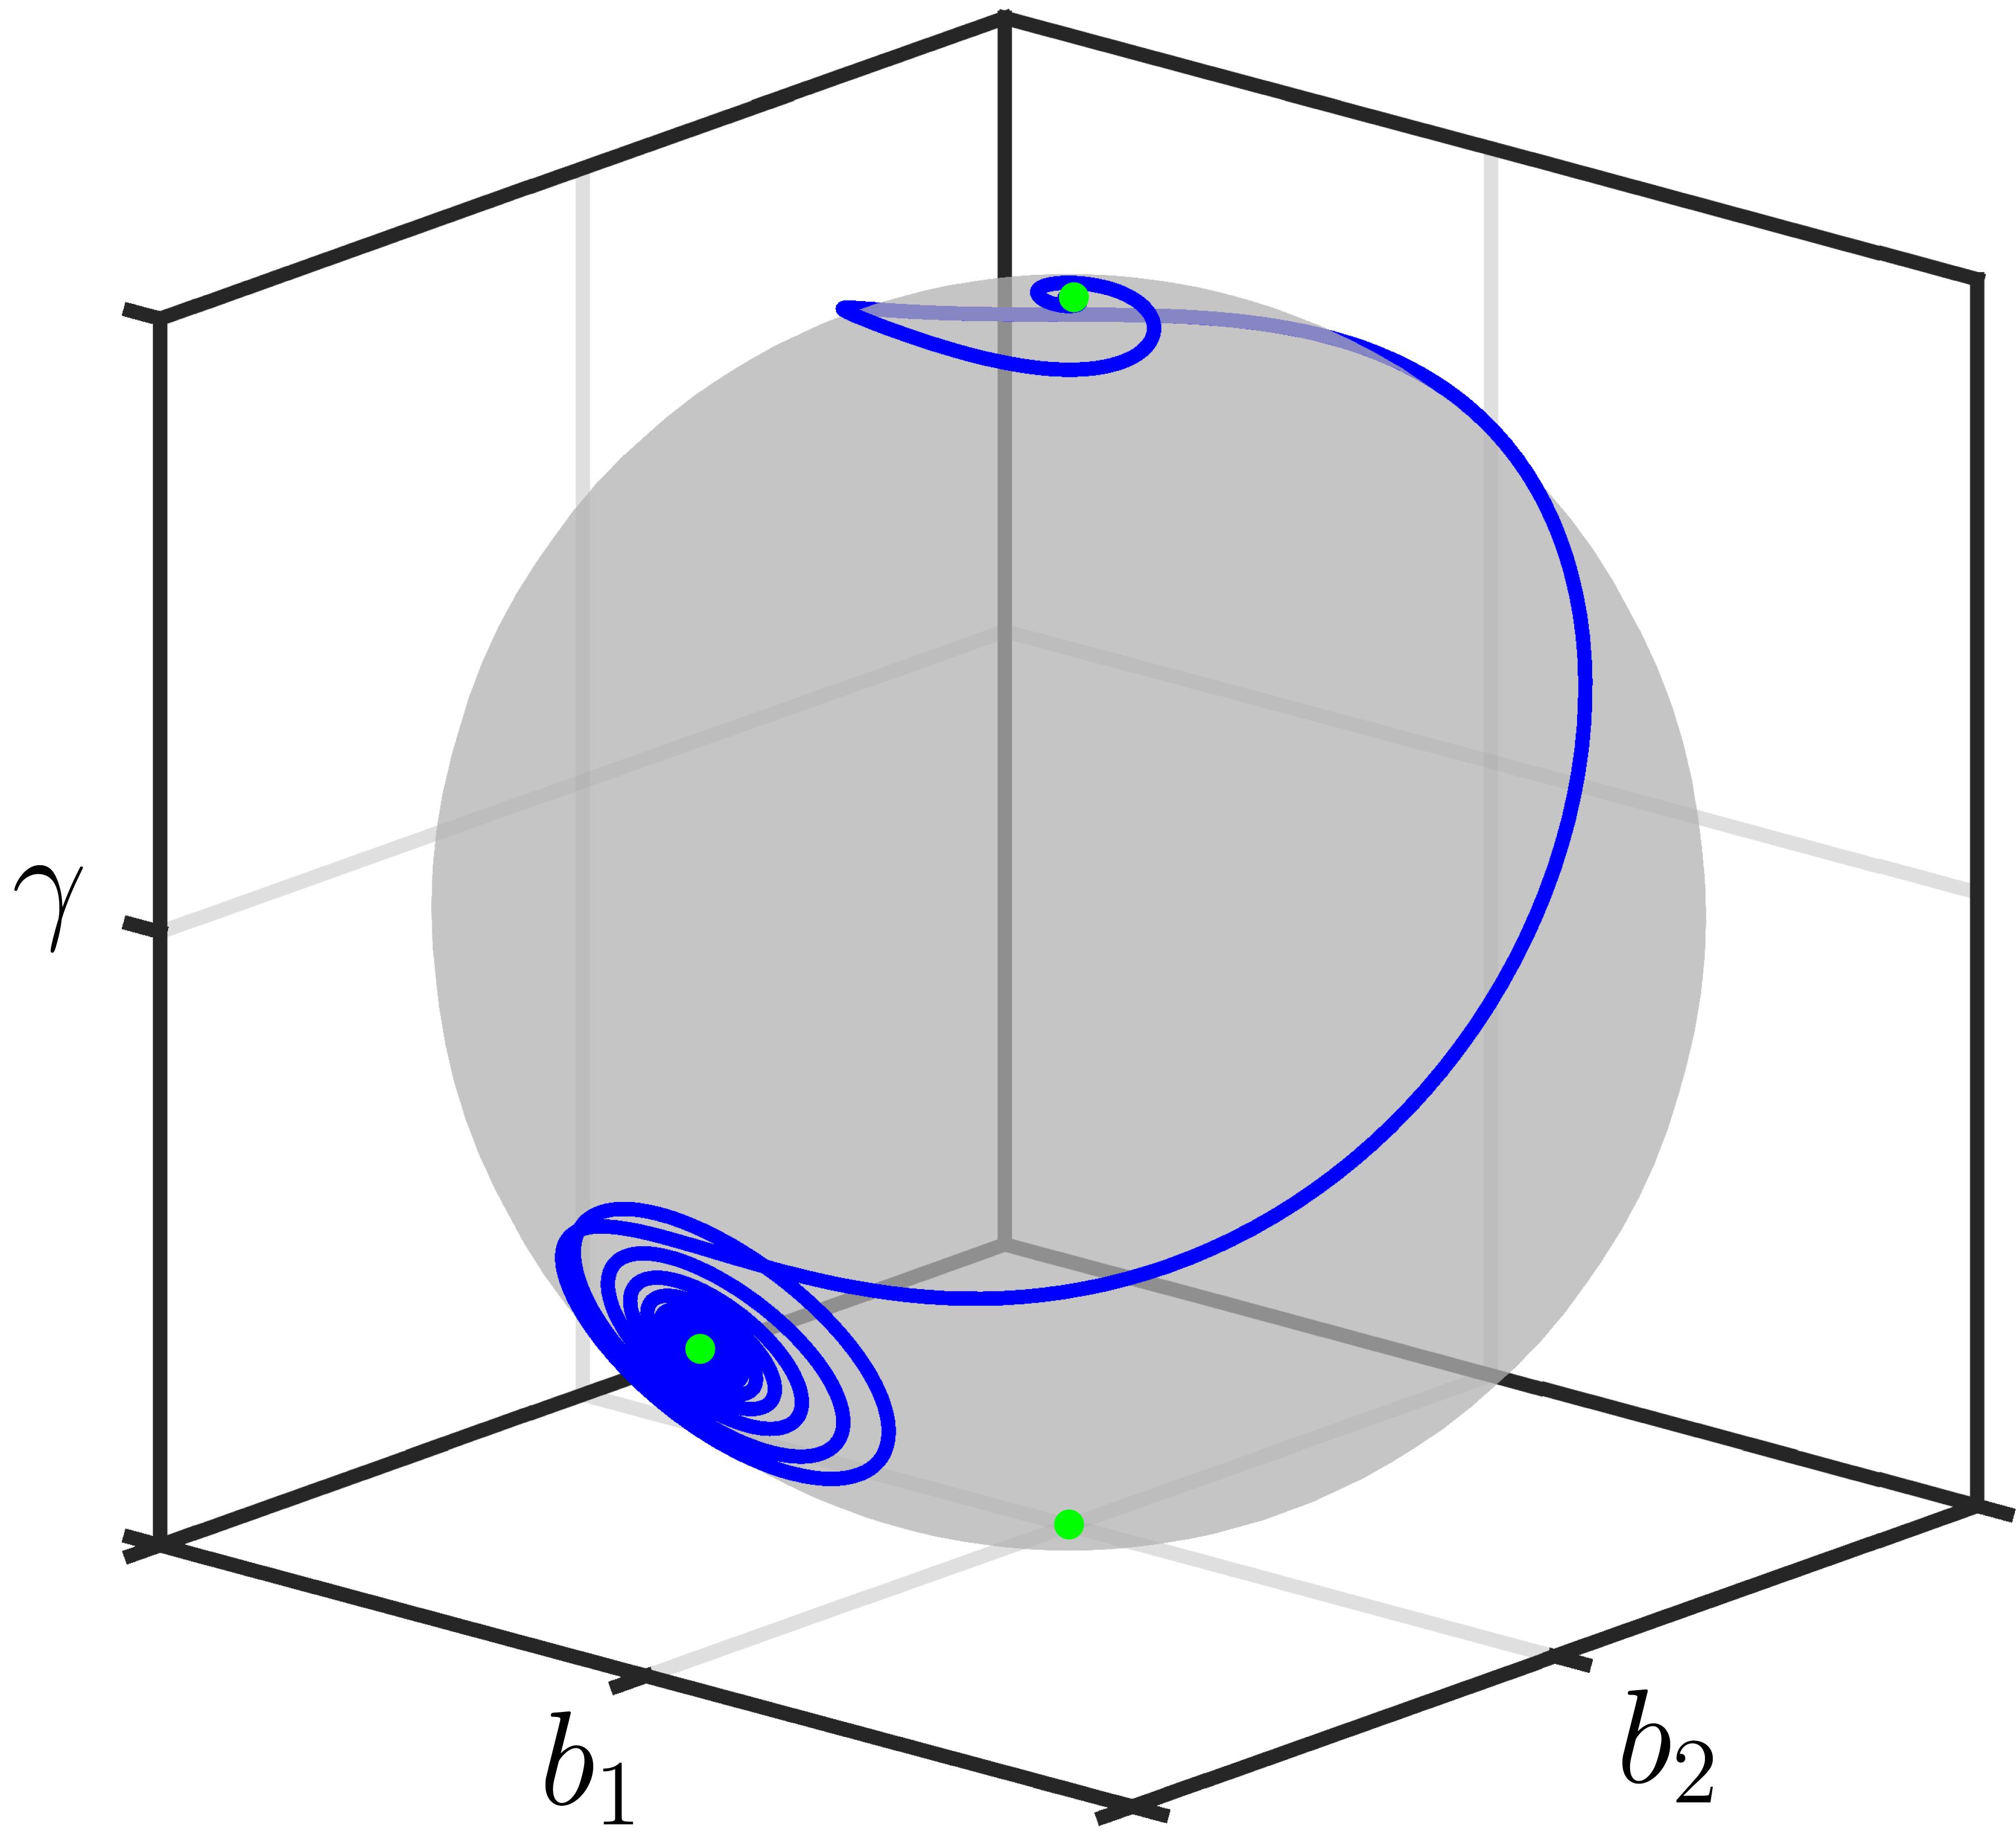
\includegraphics[width=8.6cm]{HTML_BlochSphereSprRad.eps}}
%\put(19,1){\LARGE $b_{1}$}
%\put(68,2){\LARGE $b_{2}$}
%\put(-5,41){\LARGE $\gamma$}
%
%\end{picture}
%\newpage
%
%
%\begin{picture}(100,100)
%
%\put(0,0){\includegraphics[width=8.6cm]{HTML_BlochSphereMultiNormal.eps}}
%\put(10,7){\LARGE $b_{1}$}
%\put(59.5,0.5){\LARGE $b_{2}$}
%\put(-4,49.5){\LARGE $\gamma$}
%\end{picture}
%	
%\newpage
%
%\begin{picture}(100,100)
%
%\put(0,0){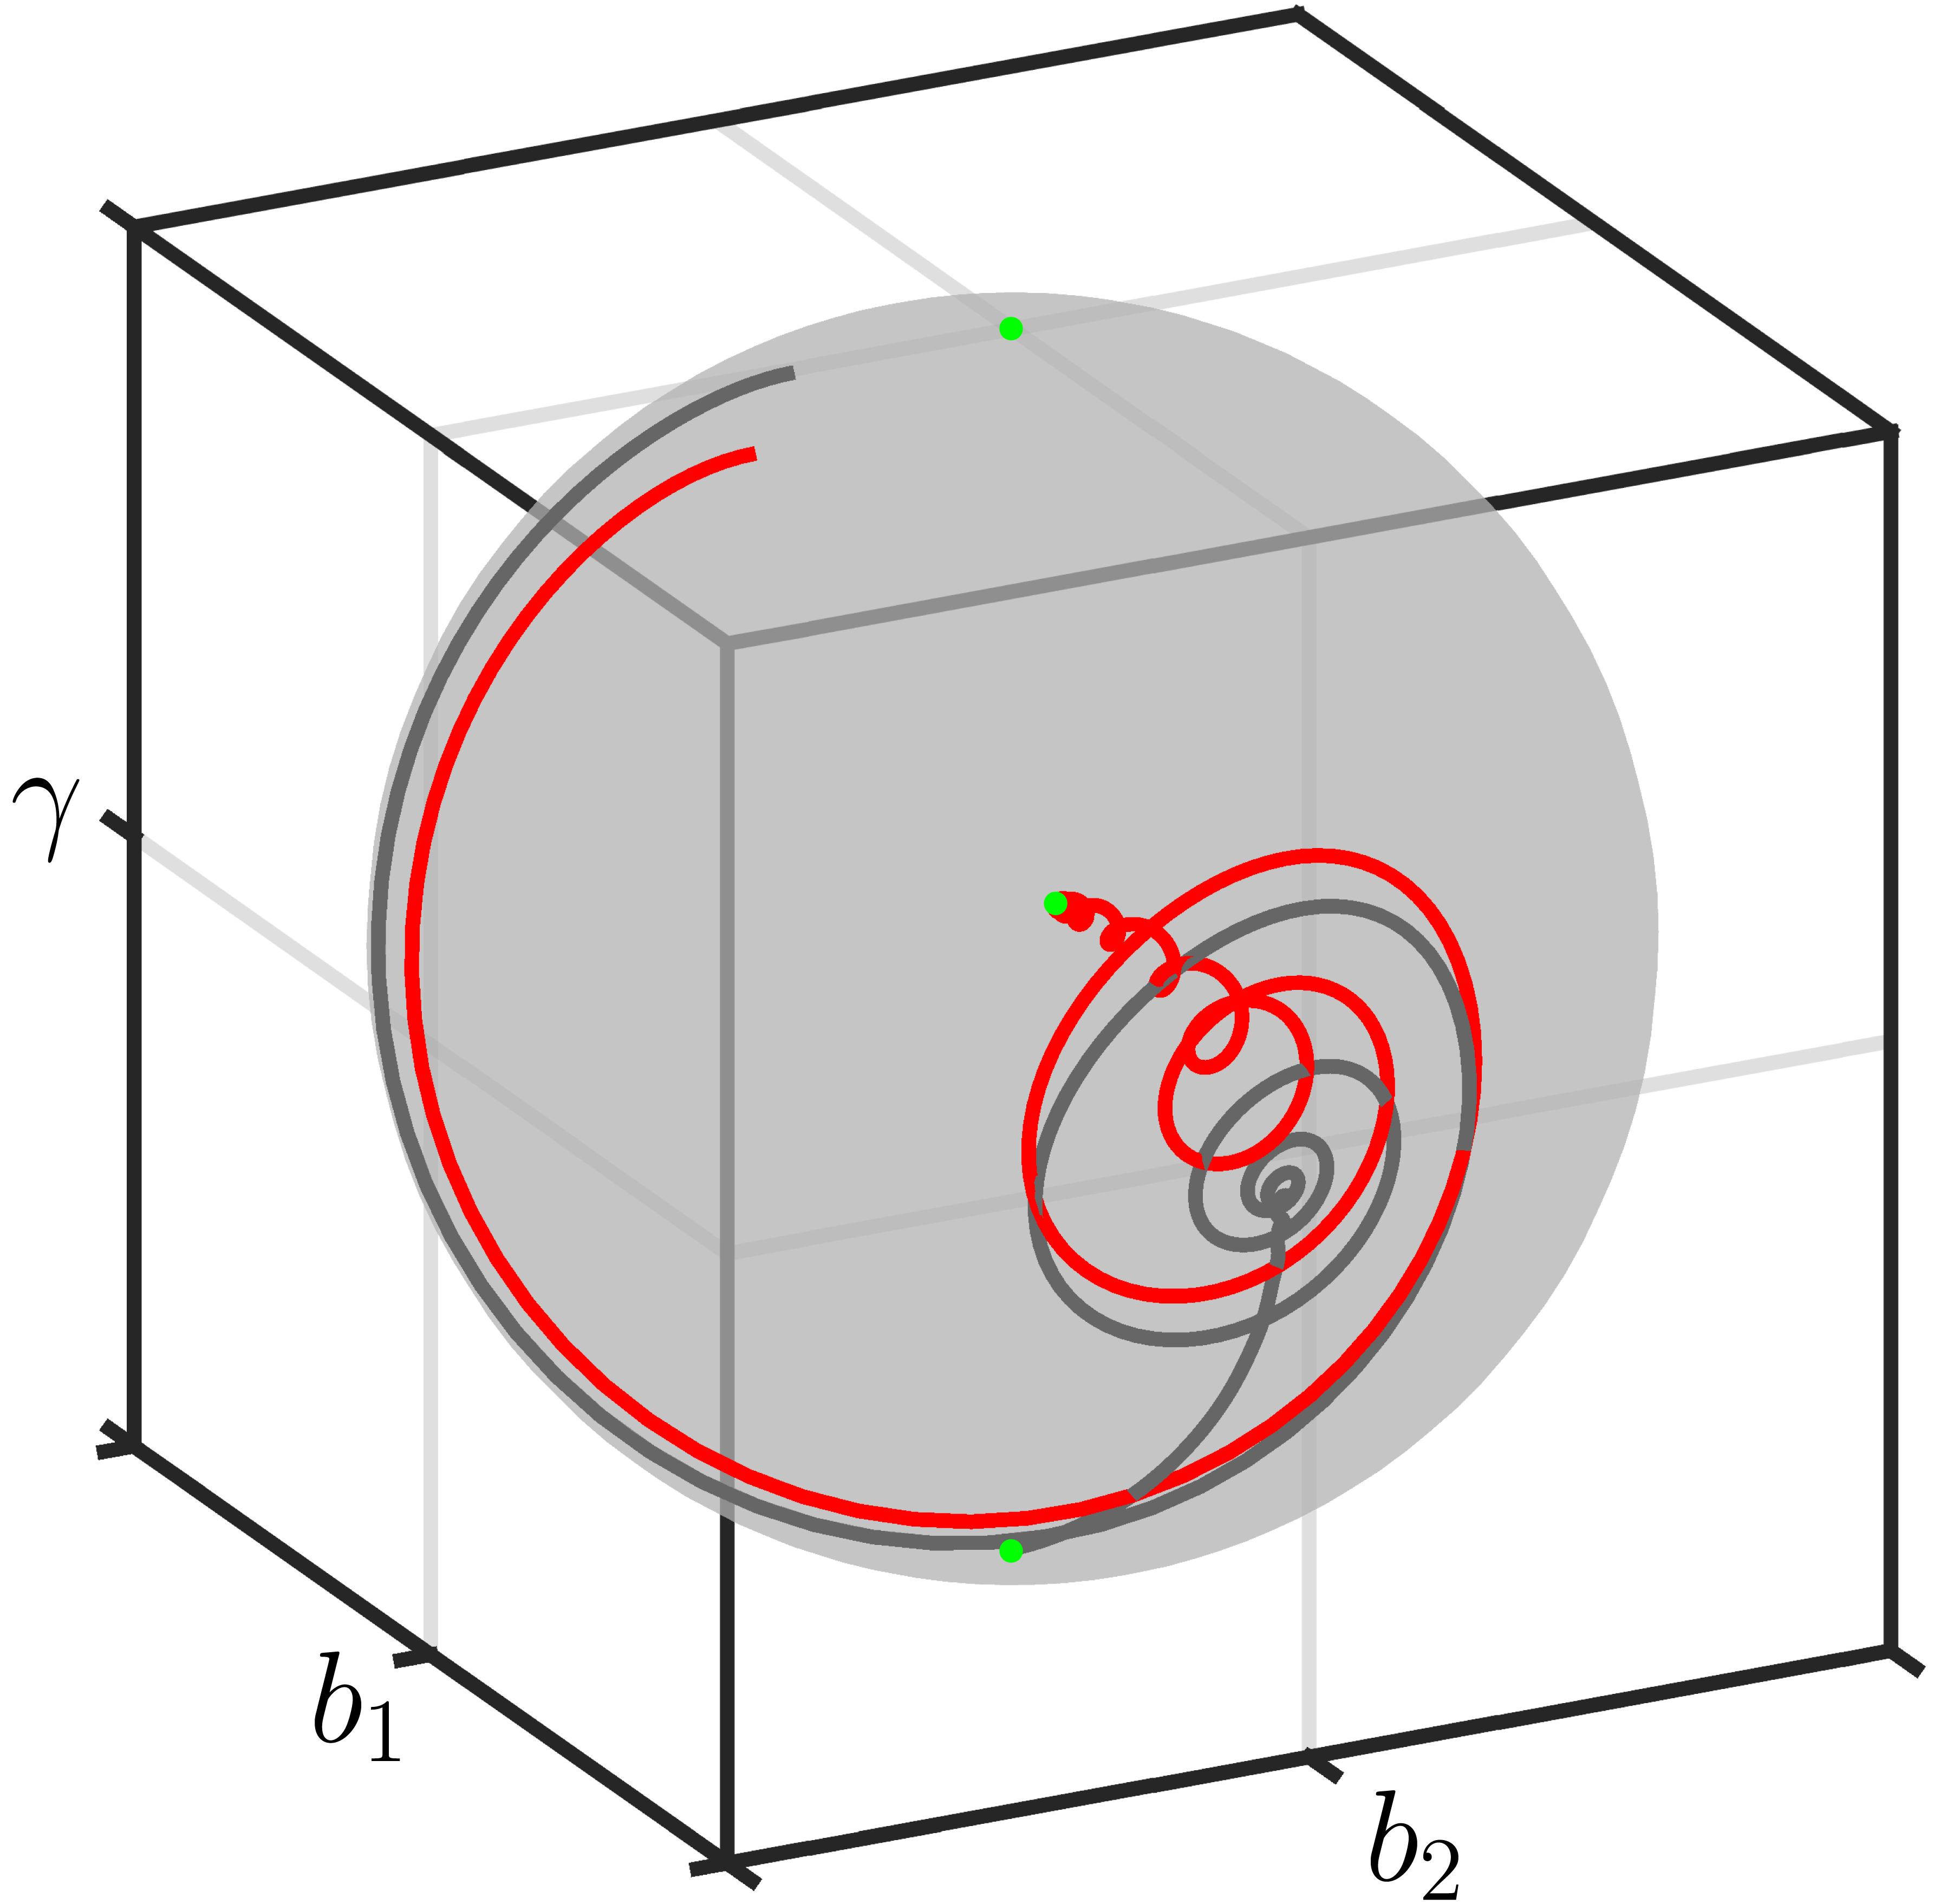
\includegraphics[width=8.6cm]{HTML_BlochSphereMultiSprRad.eps}}
%\put(10,7){\LARGE $b_{1}$}
%\put(59.5,0.5){\LARGE $b_{2}$}
%\put(-4,49.5){\LARGE $\gamma$}
%
%\end{picture}
%
%
%\newpage	
%\begin{picture}(100,100)
%
%\put(0,0){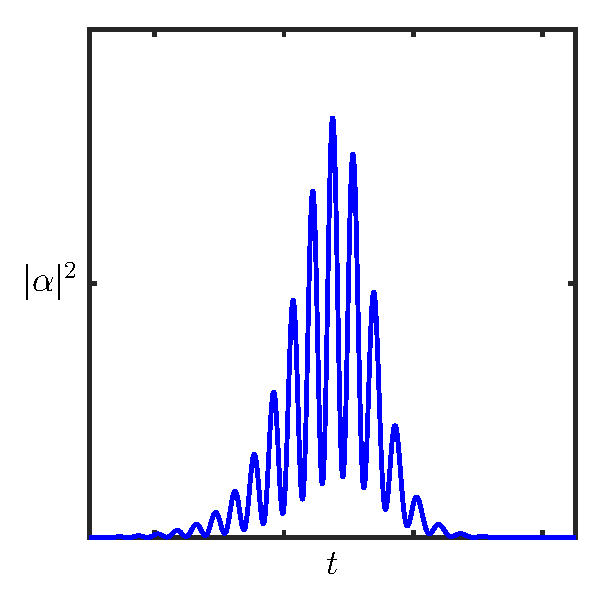
\includegraphics[width=8.6cm]{HTML_PhotonNumberNormal.eps}}
%\put(41.5,-4){\LARGE $t$}
%\put(-10,44){\LARGE $|\alpha|^2$}
%
%
%\end{picture}
%
%\newpage
%
%\begin{picture}(100,100)
%
%\put(0,0){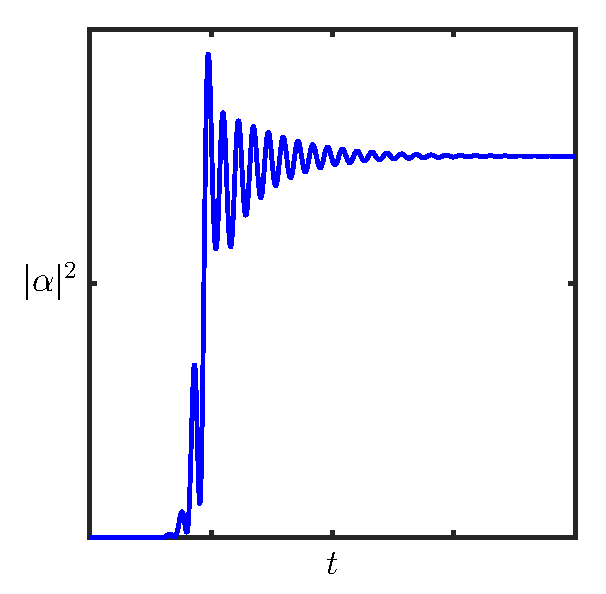
\includegraphics[width=8.6cm]{HTML_PhotonNumberSprRad.eps}}
%\put(41.5,-4){\LARGE $t$}
%\put(-10,44){\LARGE $|\alpha|^2$}
%
%\end{picture}
%
%\newpage
%
%\begin{picture}(100,100)
%
%\put(0,0){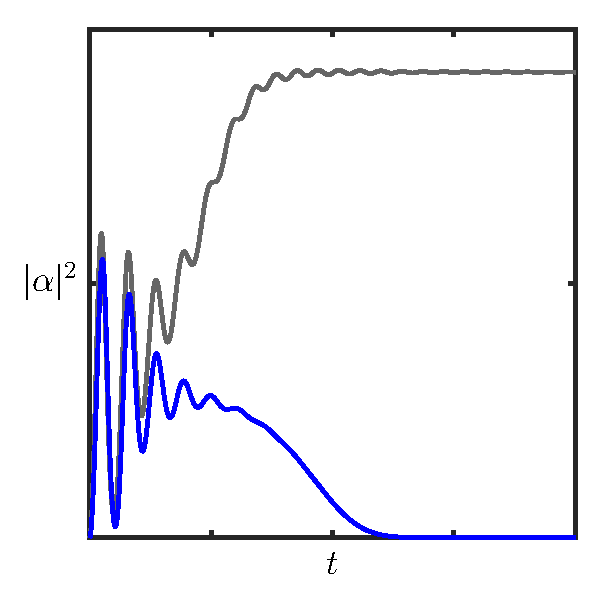
\includegraphics[width=8.6cm]{HTML_PhotonNumberMultiNormal.eps}}
%\put(41.5,-4){\LARGE $t$}
%\put(-10,44){\LARGE $|\alpha|^2$}
%
%\end{picture}
%\newpage
%
%\begin{picture}(100,100)
%
%\put(0,0){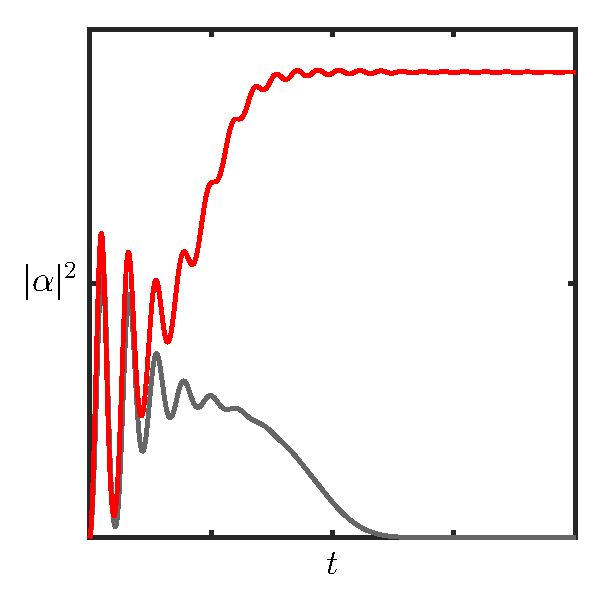
\includegraphics[width=8.6cm]{HTML_PhotonNumberMultiSprRad.eps}}
%\put(41.5,-4){\LARGE $t$}
%\put(-10,44){\LARGE $|\alpha|^2$}
%
%\end{picture}
%
%
%\newpage

\begin{picture}(100,200)
\put(0,0){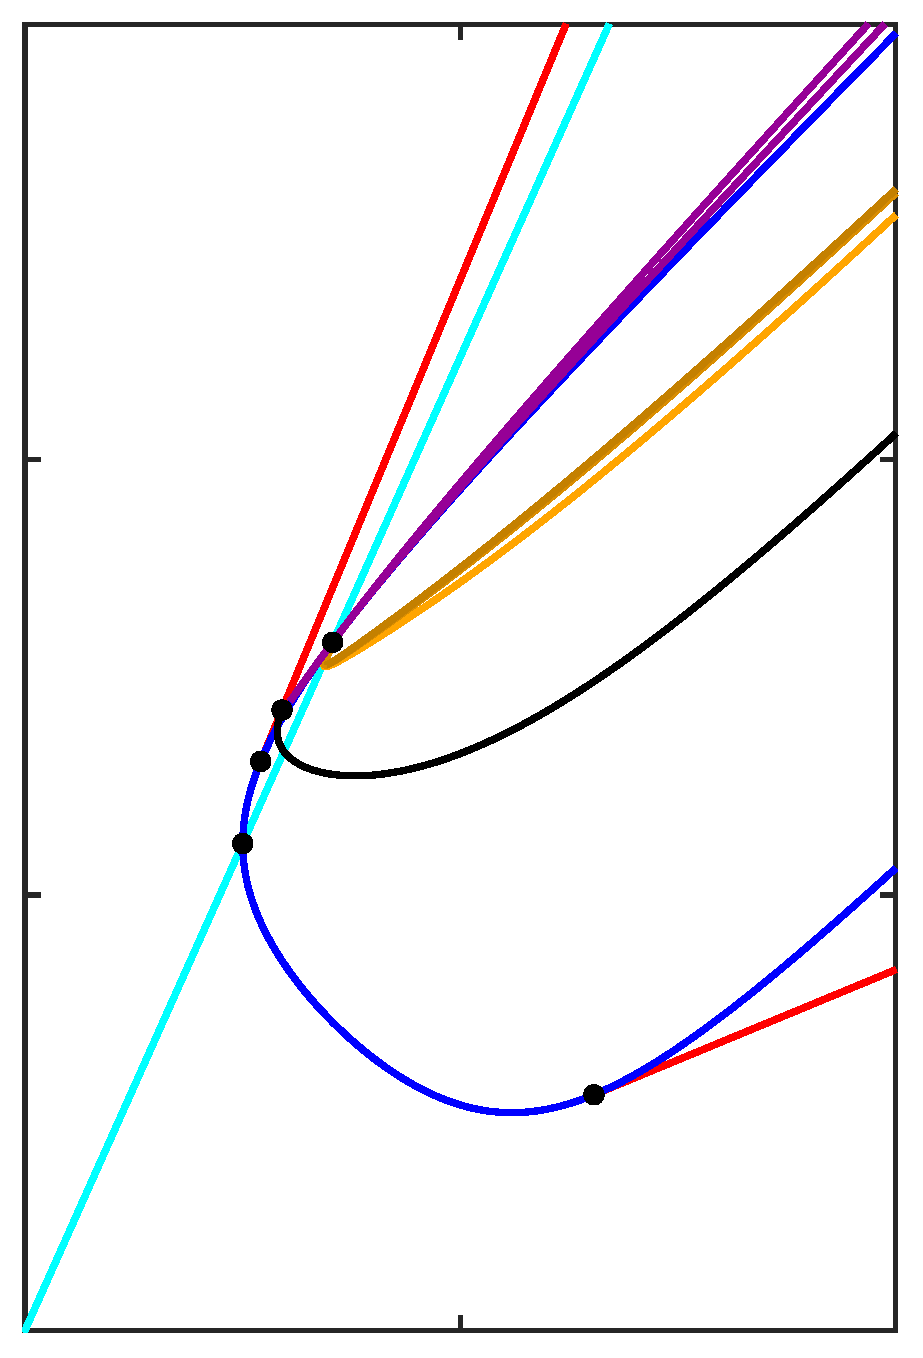
\includegraphics{HTML_BigOlePhaseDiagram.eps}}
\put(73,-5){\LARGE $\lambda_{-}$}
\put(-9,110){\LARGE $\lambda_{+}$}

\end{picture}


\newpage


\begin{picture}(100,100)

\put(0,0){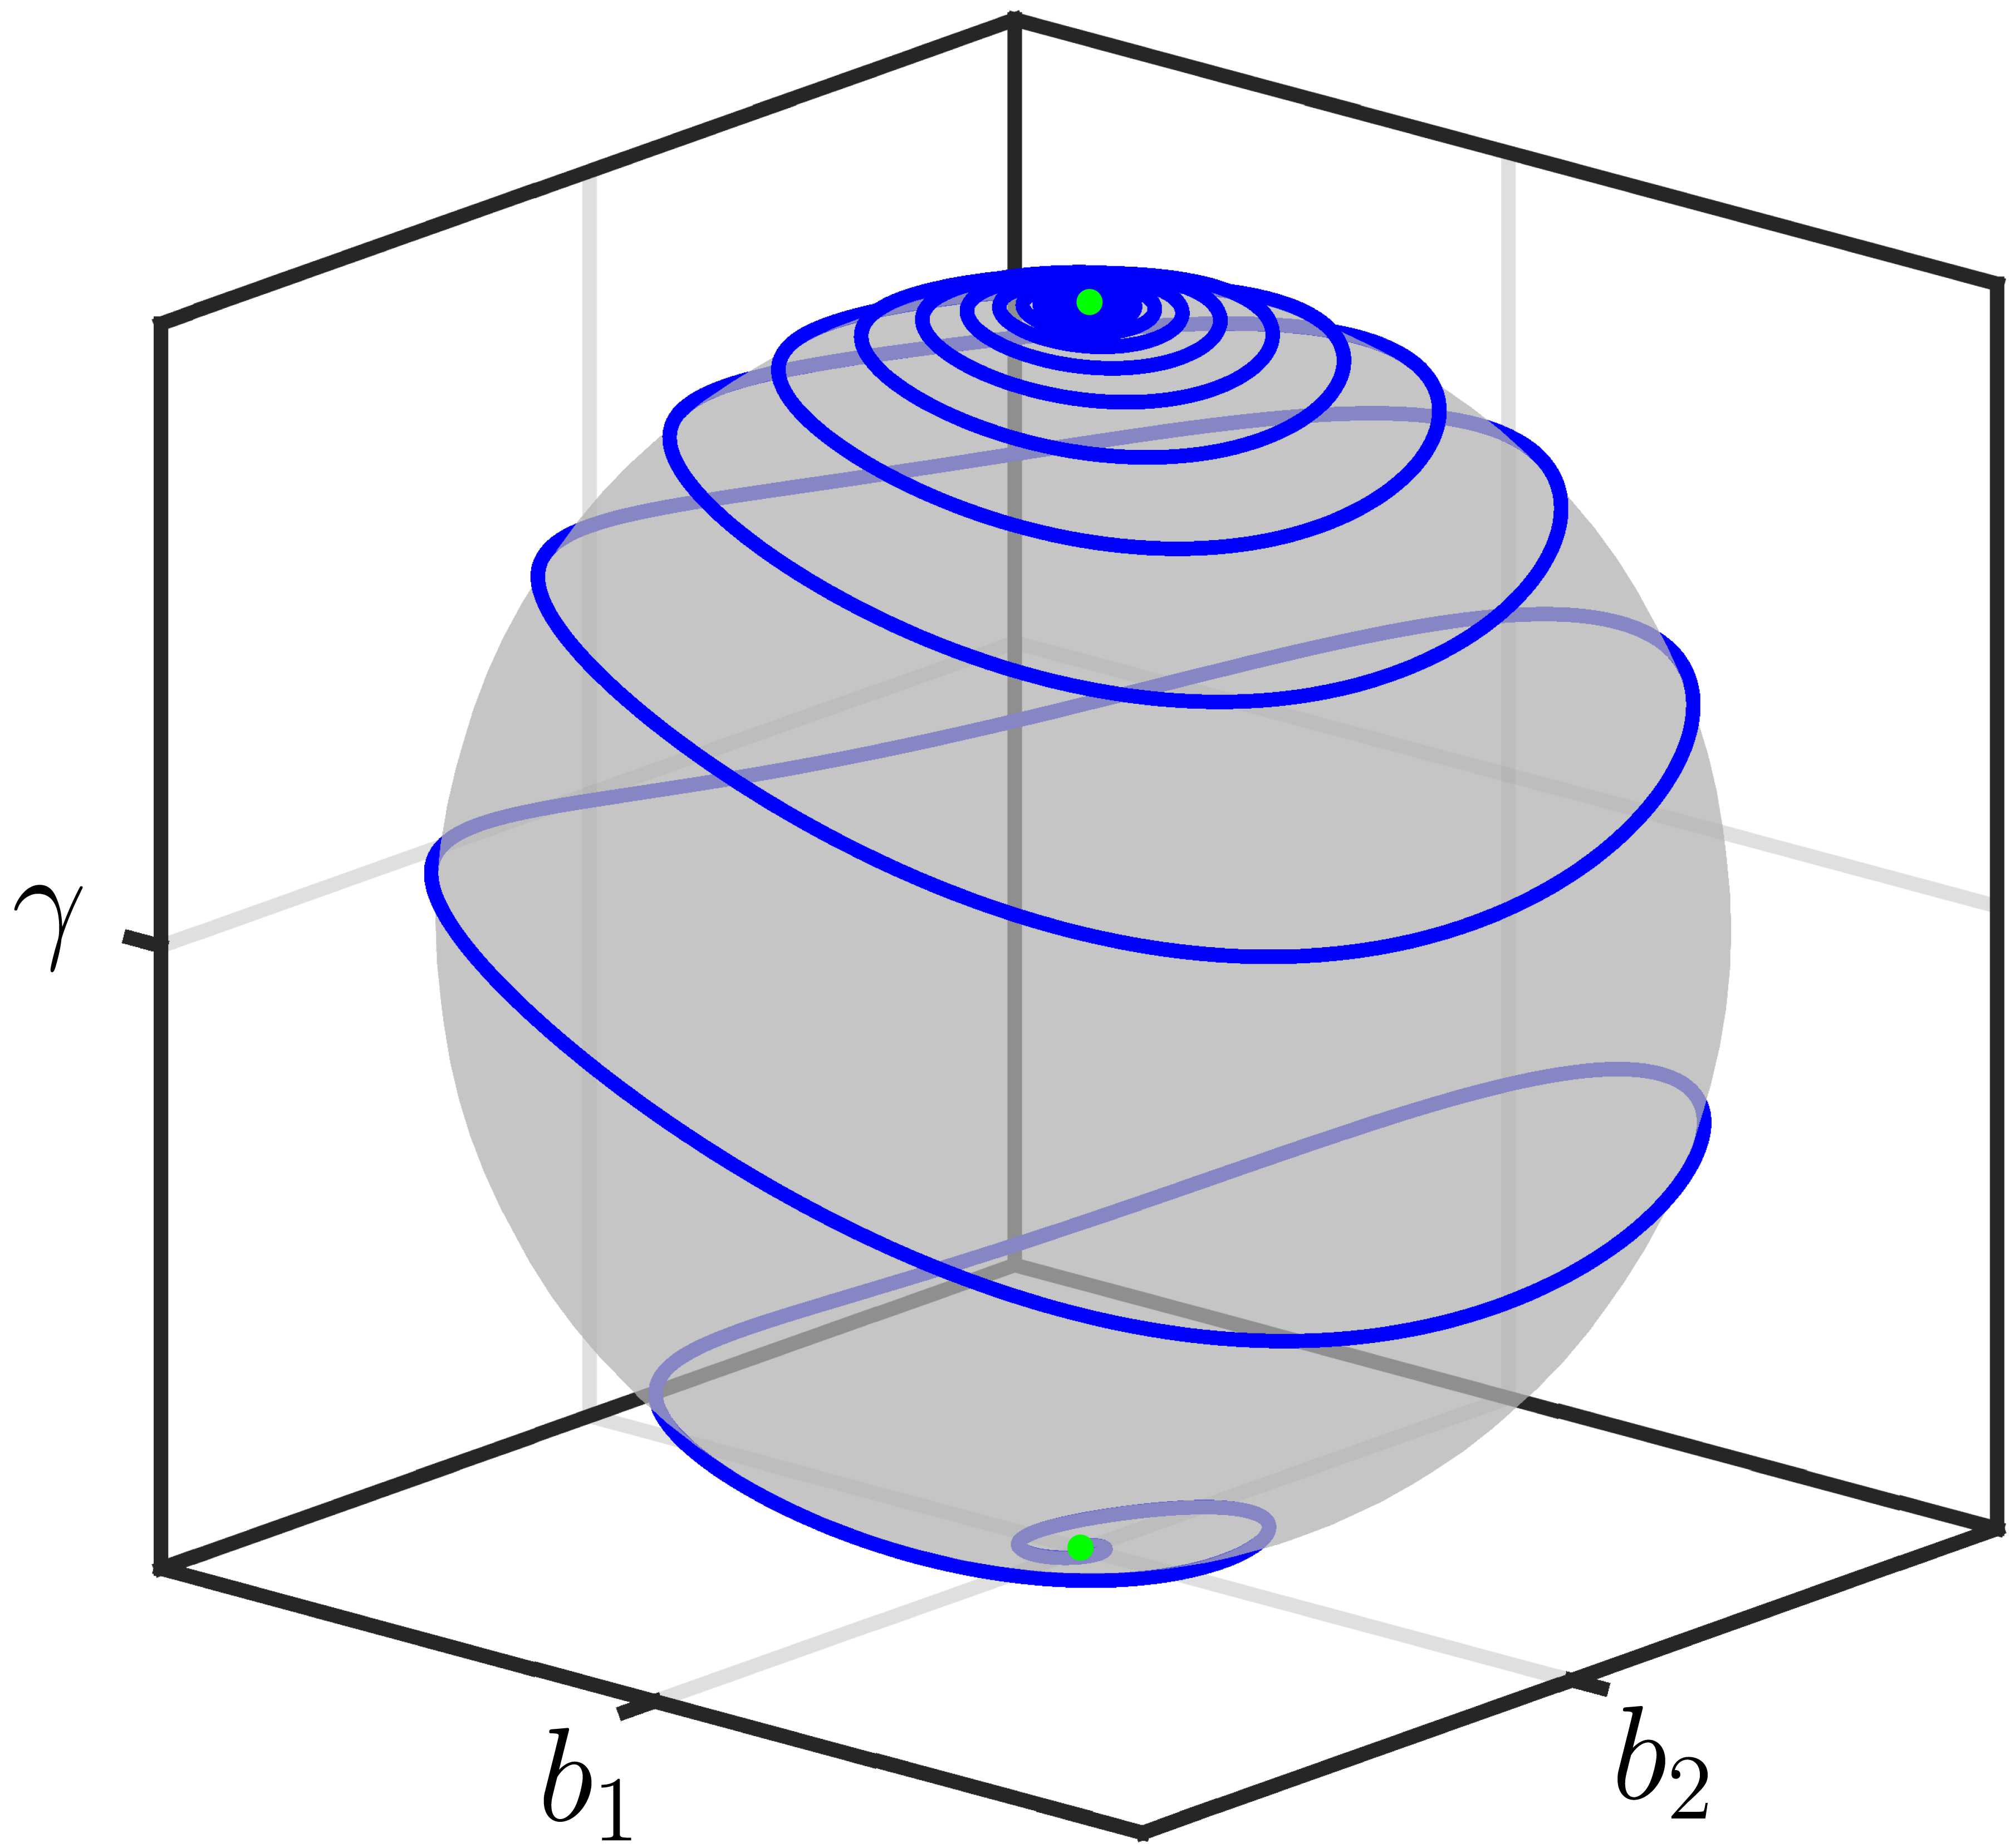
\includegraphics[width=8.6cm]{HTML_BlochSphereUpNormal.eps}}
\put(19,1){\LARGE $b_{1}$}
\put(68,2){\LARGE $b_{2}$}
\put(-5,41){\LARGE $\gamma$}

\end{picture}


\newpage
\begin{picture}(100,100)
\put(0,0){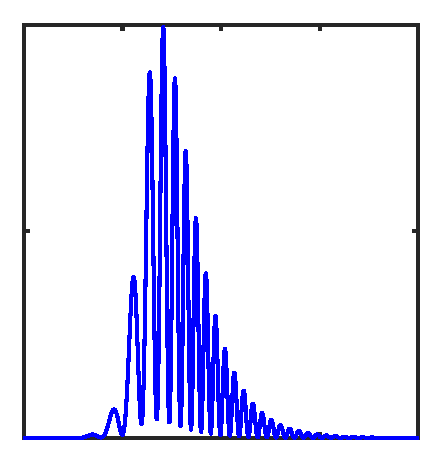
\includegraphics[width=8.6cm]{HTML_PhotonNumberUpNormal.eps}}
\put(41.5,-4){\LARGE $t$}
\put(-10,44){\LARGE $|\alpha|^2$}

\end{picture}

\newpage

\begin{picture}(100,100)

\put(0,0){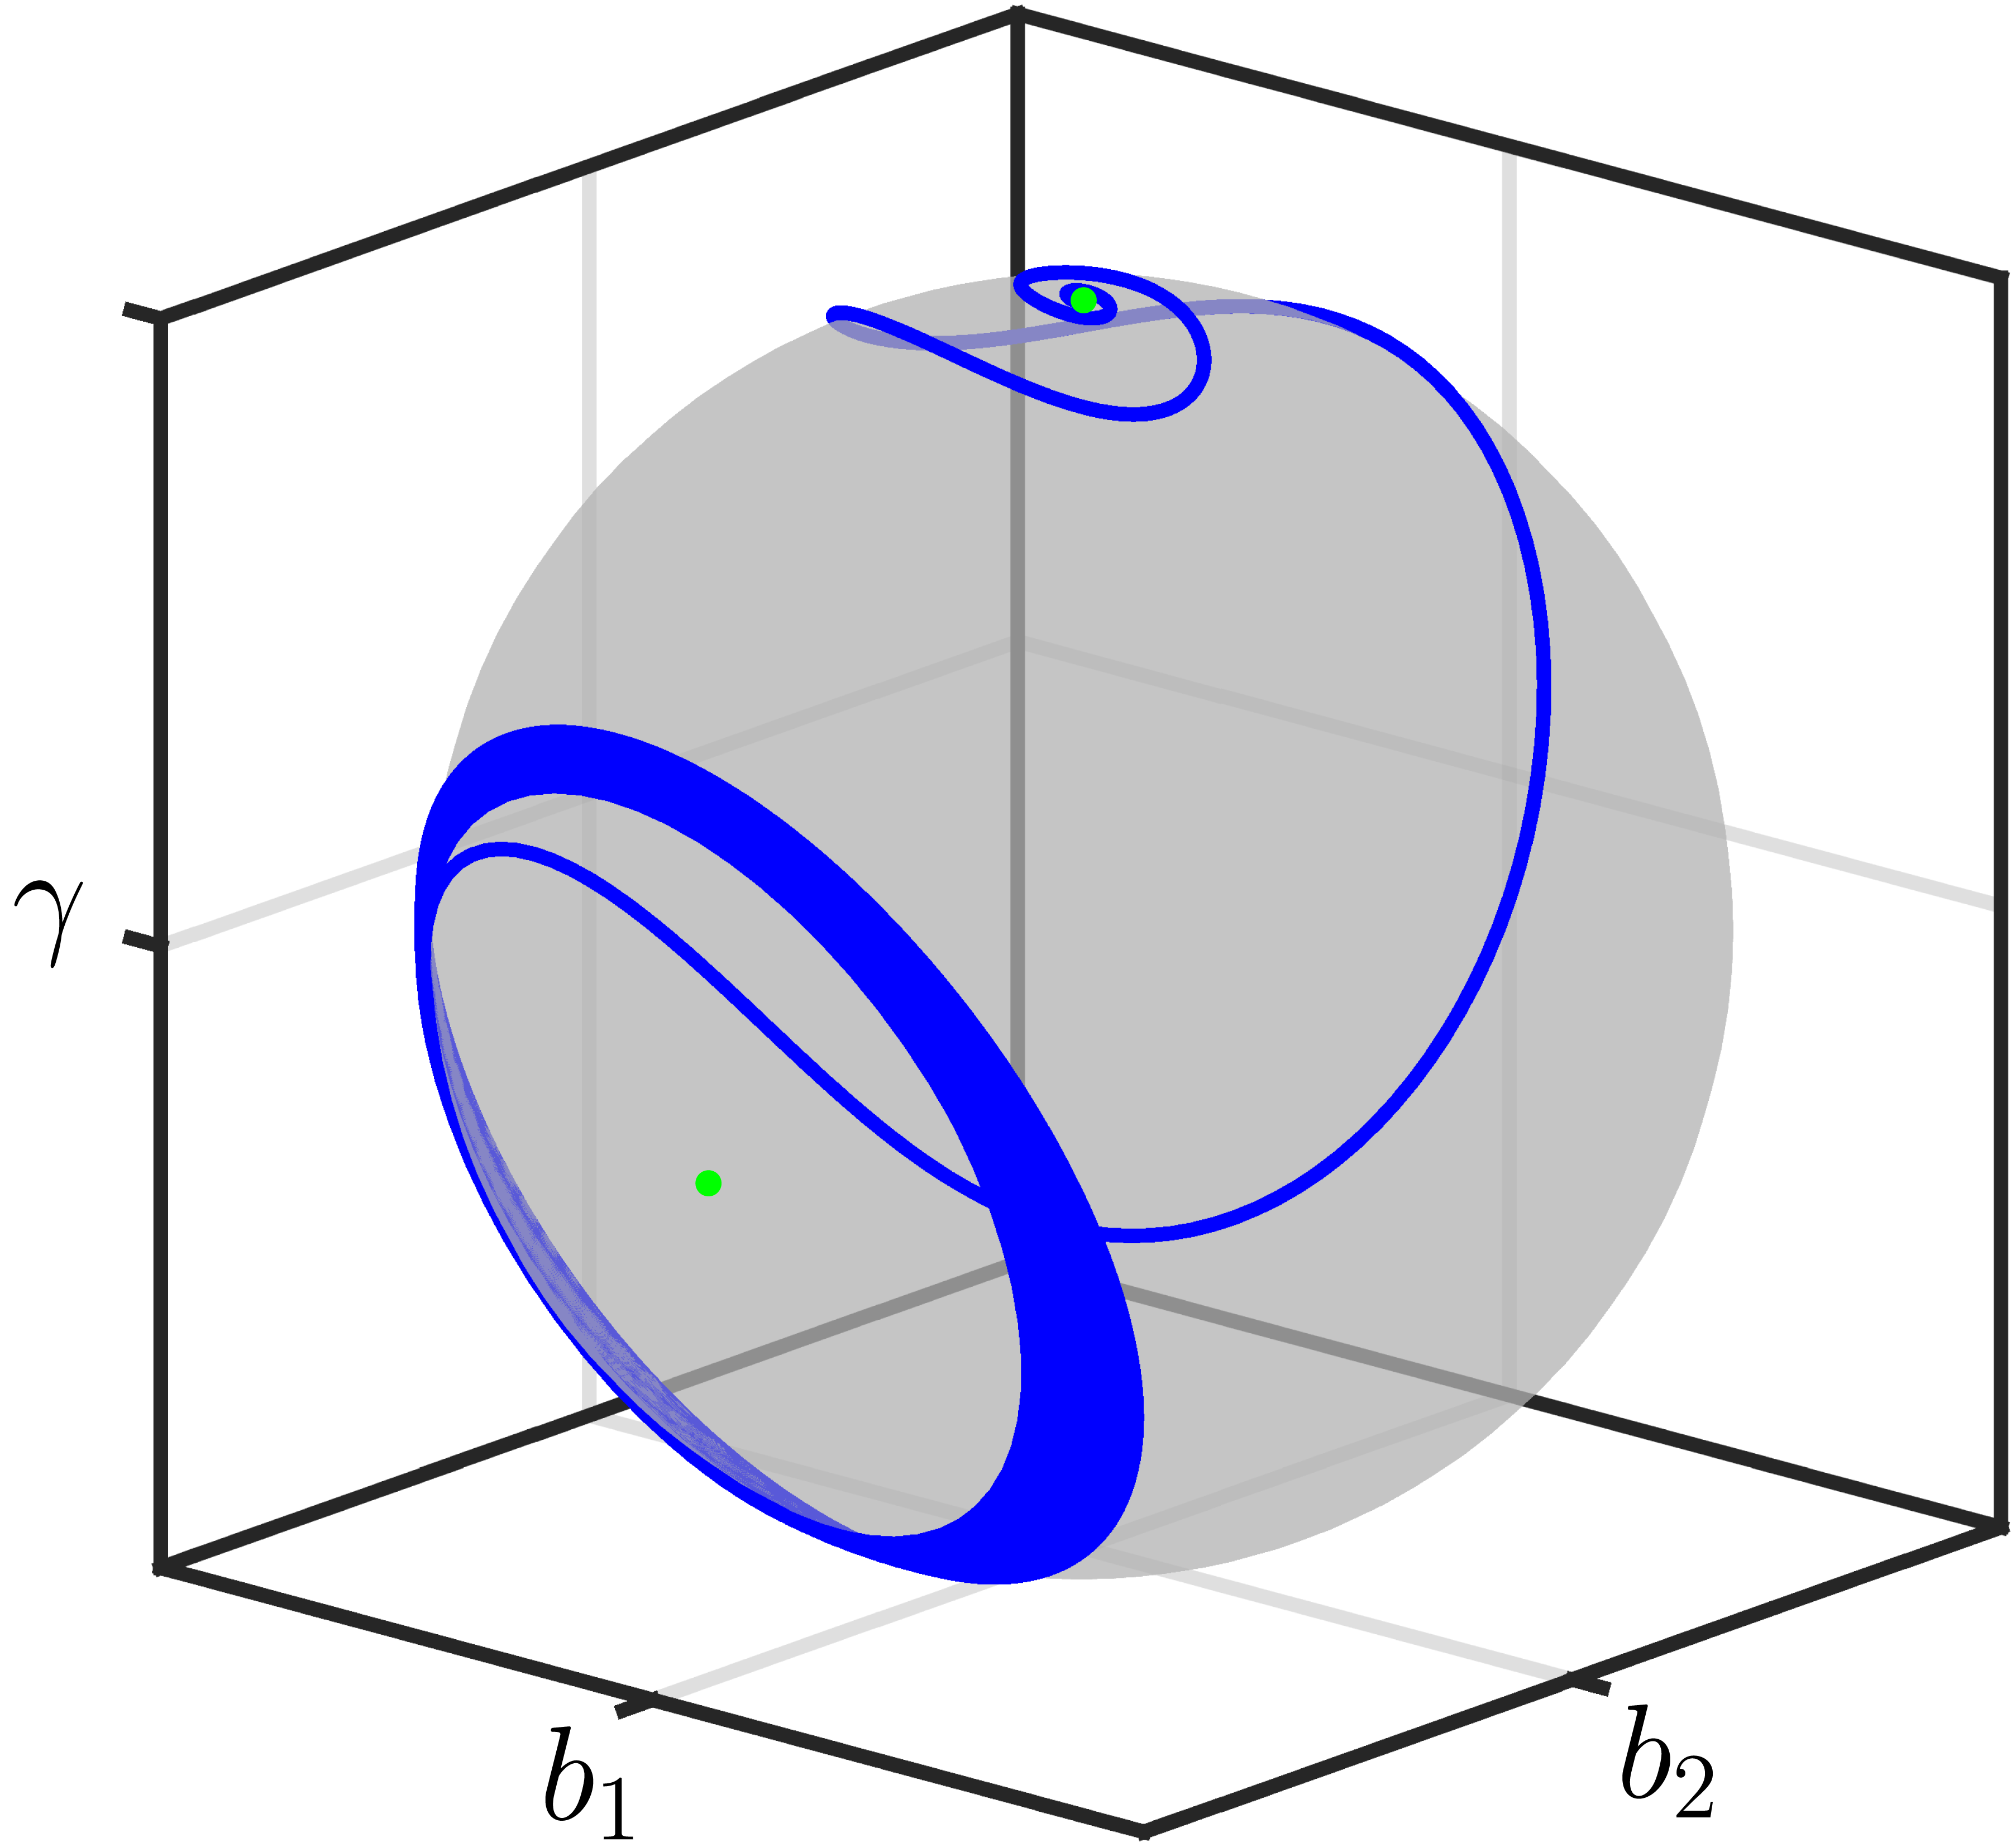
\includegraphics[width=8.6cm]{HTML_BlochSphereOscillation.eps}}
\put(19,1){\LARGE $b_{1}$}
\put(68,2){\LARGE $b_{2}$}
\put(-5,41){\LARGE $\gamma$}
\end{picture}

\newpage

\begin{picture}(100,100)
\put(0,0){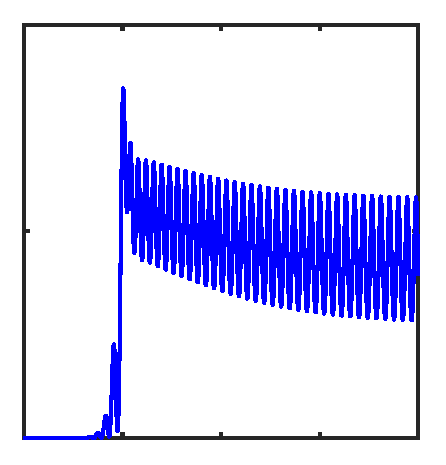
\includegraphics[width=8.6cm]{HTML_PhotonNumberOscillation.eps}}
\put(41.5,-4){\LARGE $t$}
\put(-10,44){\LARGE $|\alpha|^2$}

\end{picture}


\newpage

\begin{picture}(100,100)

\put(0,0){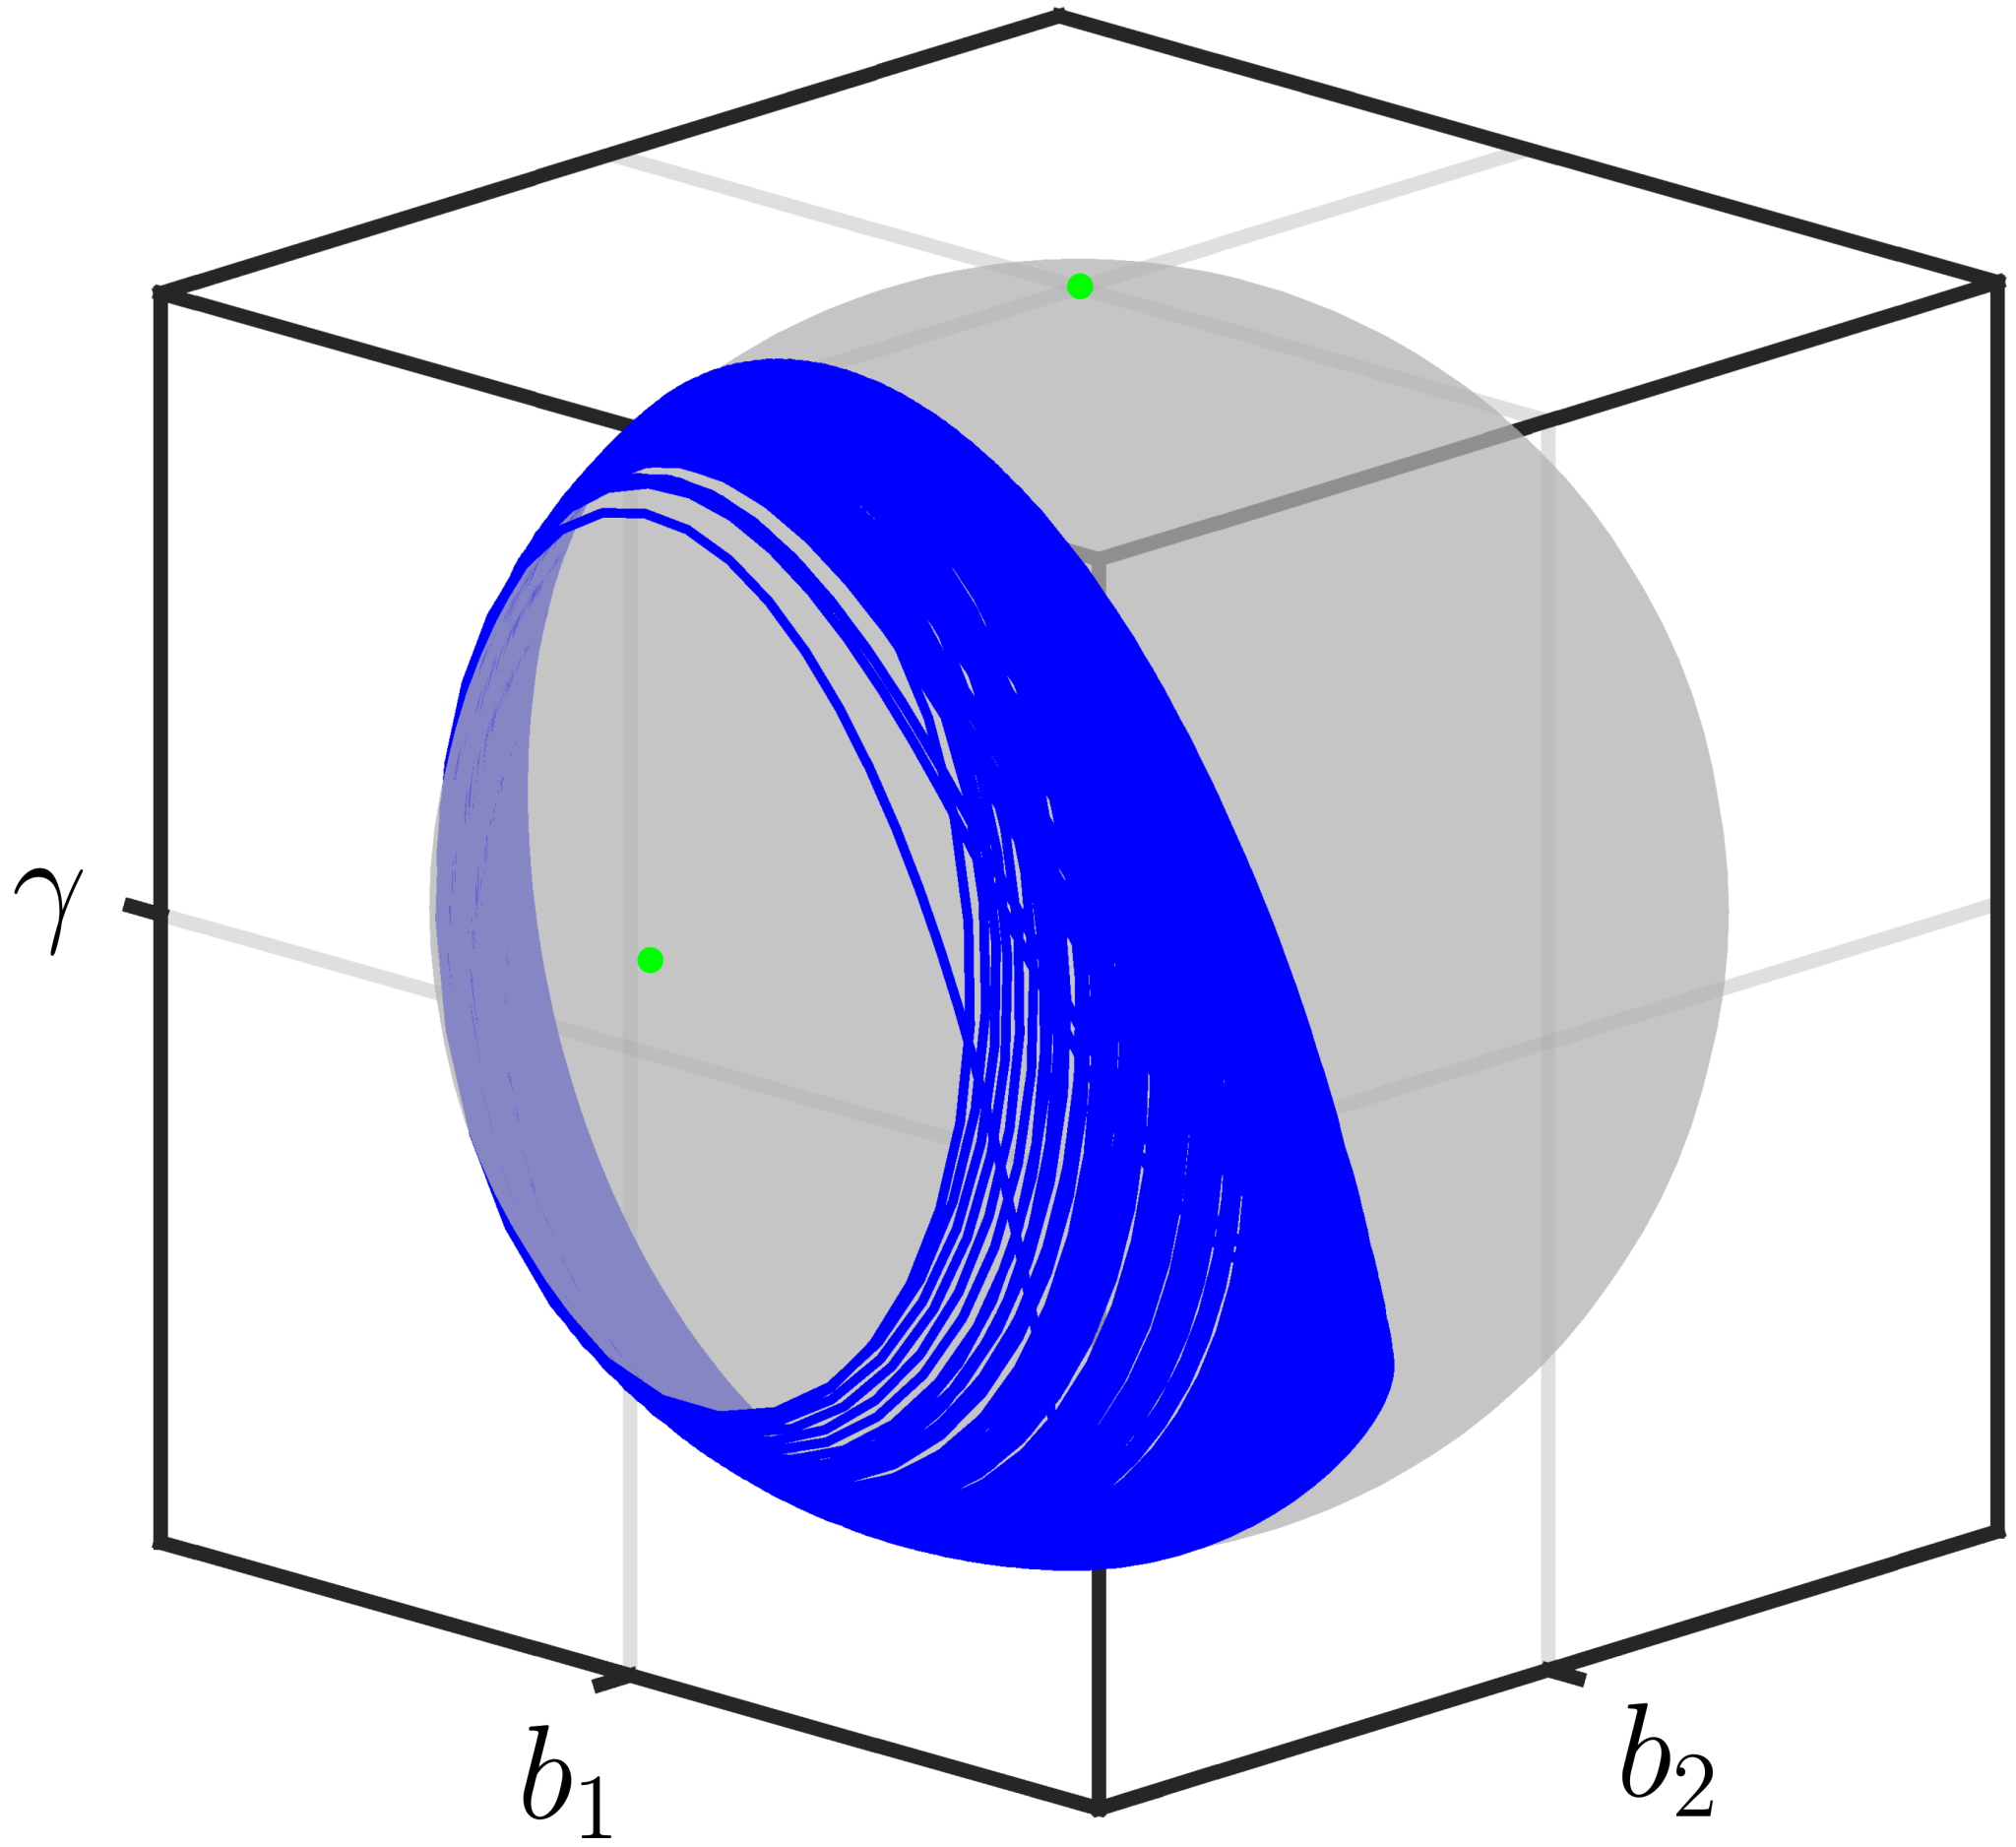
\includegraphics[width=8.6cm]{HTML_BlochSphereChaos1.eps}}
\put(18,0){\LARGE $b_{1}$}
\put(68,1){\LARGE $b_{2}$}
\put(-5,40.5){\LARGE $\gamma$}
\end{picture}


\newpage

\begin{picture}(100,100)

\put(0,0){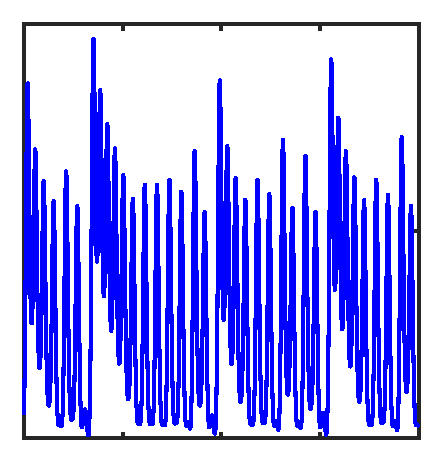
\includegraphics[width=8.6cm]{HTML_PhotonNumberChaos1.eps}}
\put(41.5,-4){\LARGE $t$}
\put(-10,44){\LARGE $|\alpha|^2$}
\end{picture}

\newpage

\begin{picture}(100,100)

\put(0,0){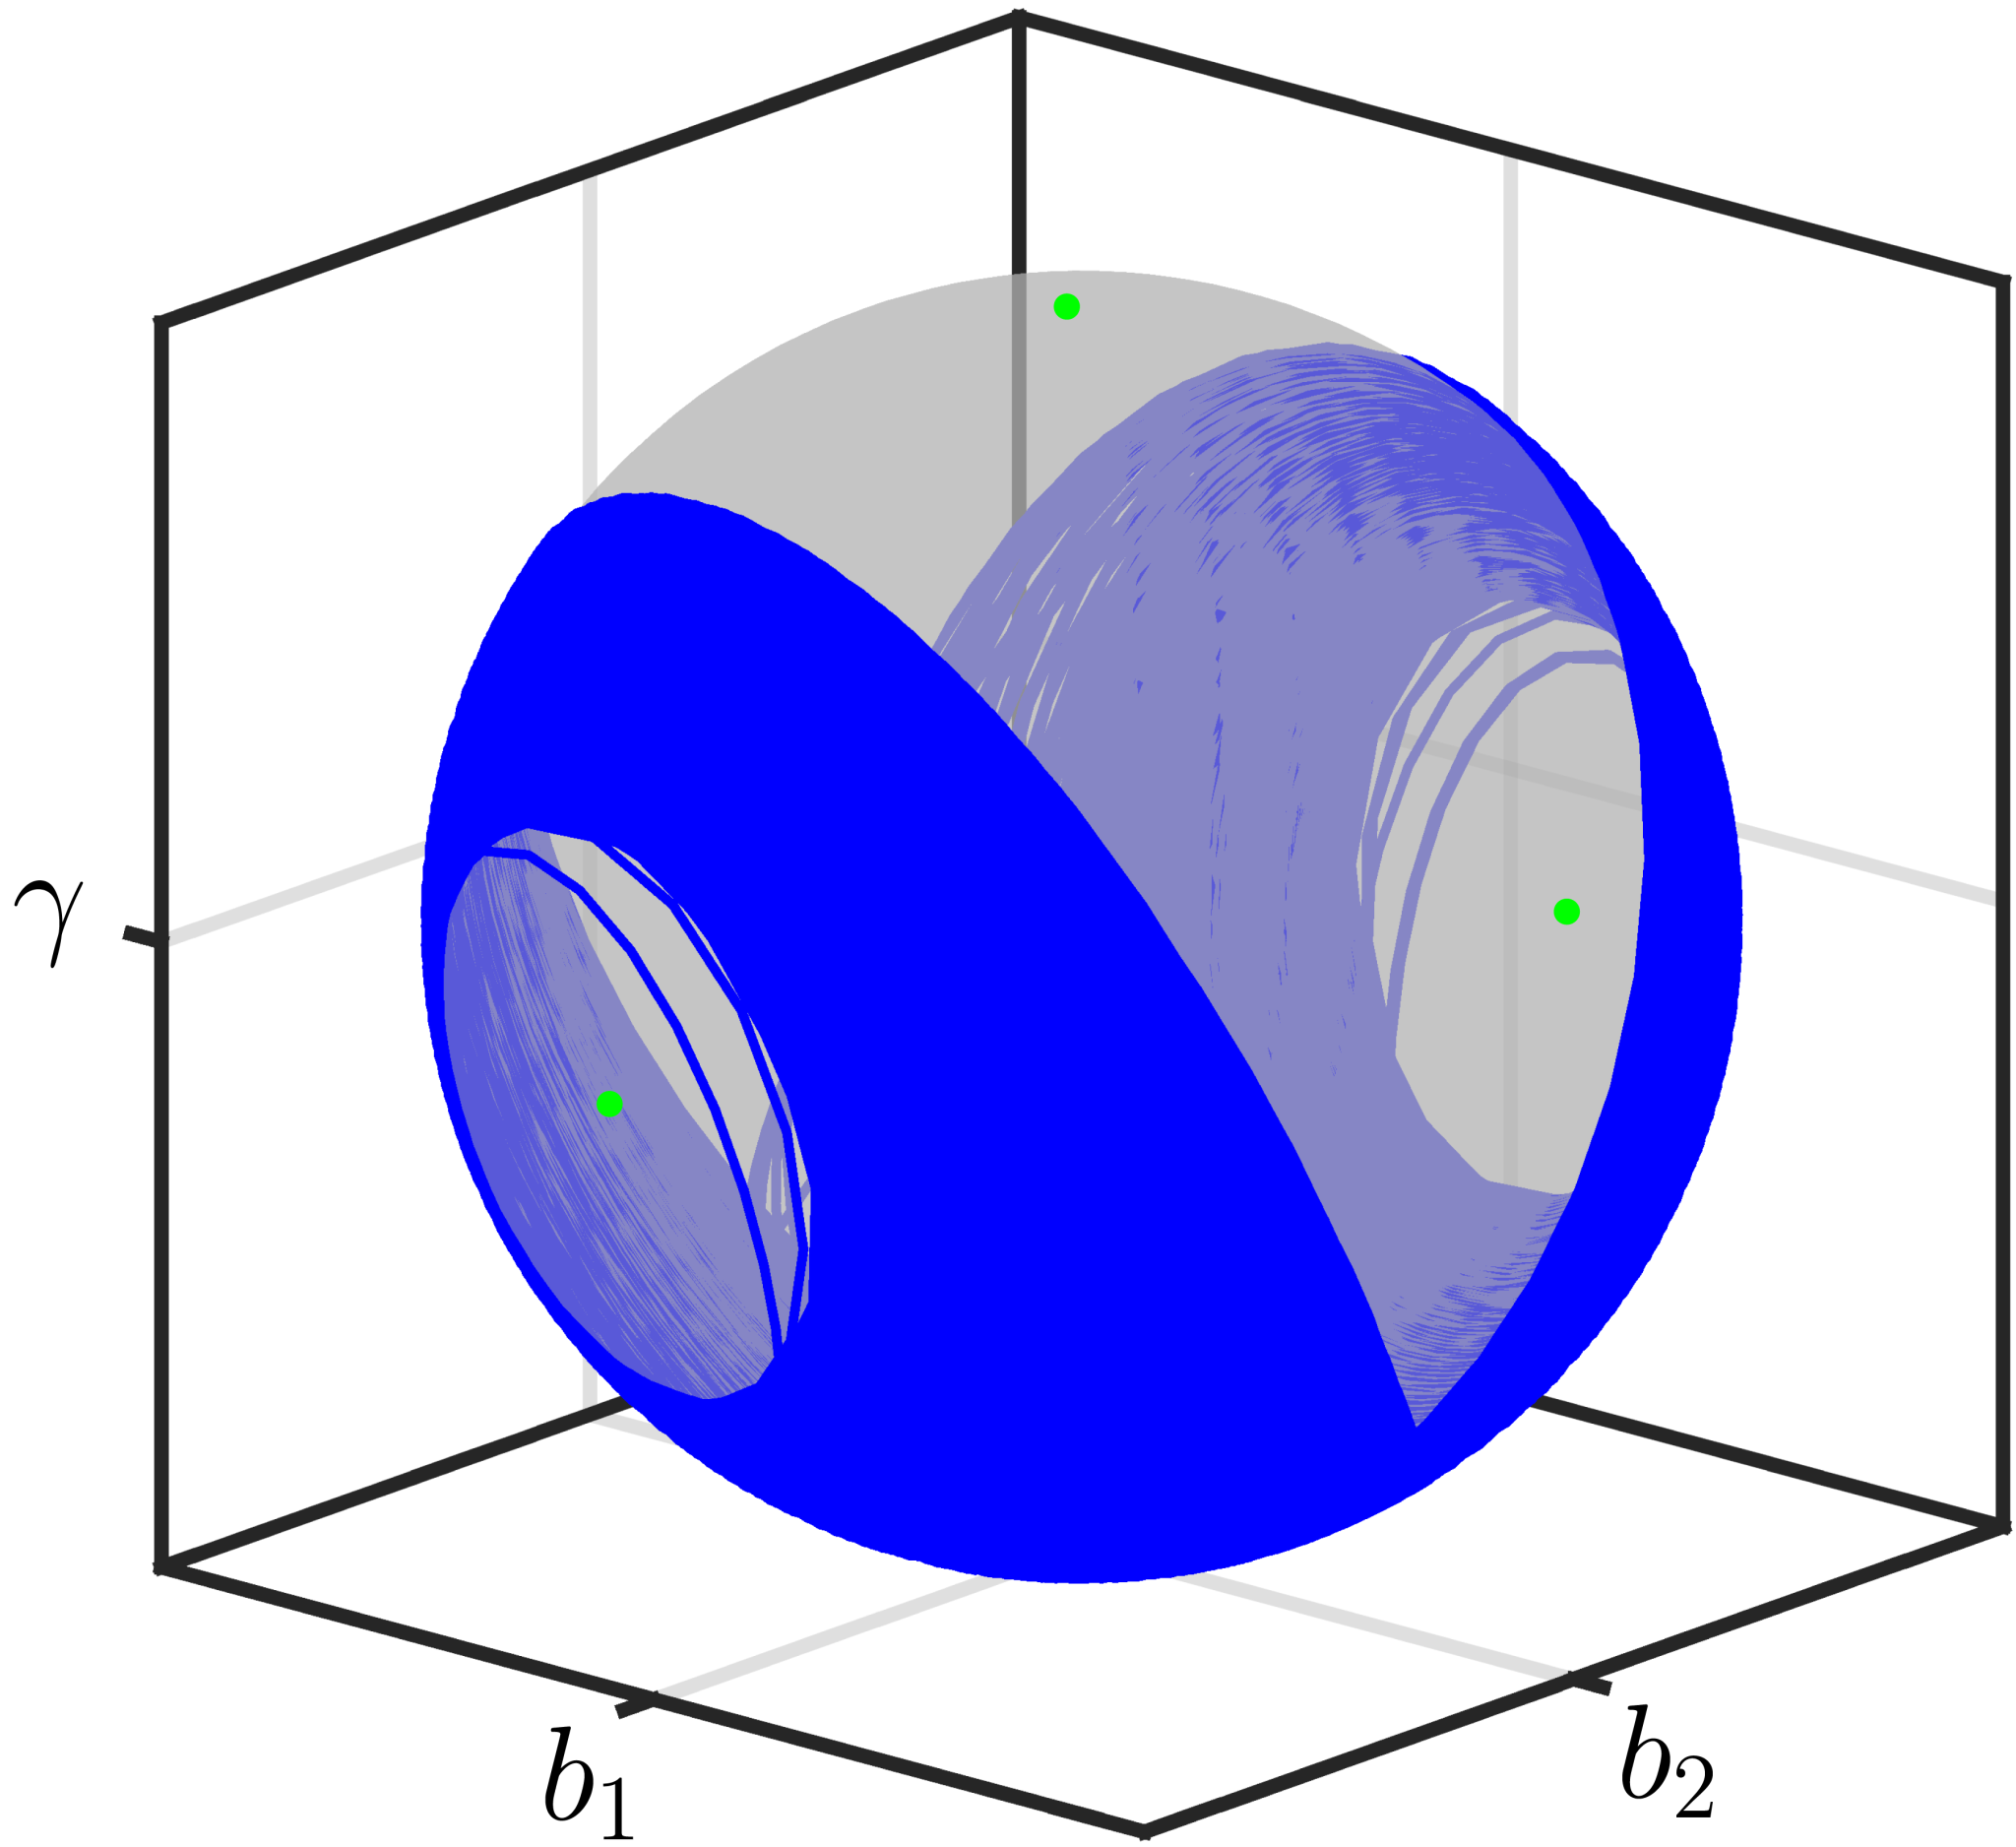
\includegraphics[width=8.6cm]{HTML_BlochSphereChaos2.eps}}
\put(19,1){\LARGE $b_{1}$}
\put(68,2){\LARGE $b_{2}$}
\put(-5,41){\LARGE $\gamma$}
\end{picture}



\newpage
\begin{picture}(100,100)
\put(0,0){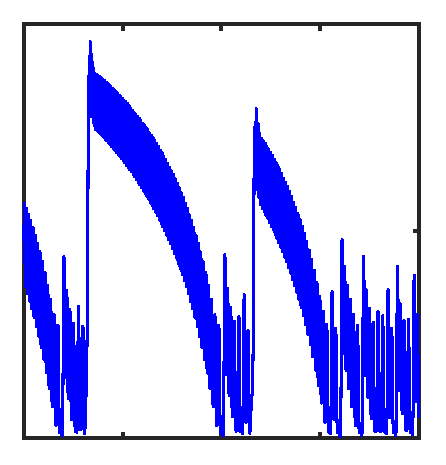
\includegraphics[width=8.6cm]{HTML_PhotonNumberChaos2.eps}}
\put(41.5,-4){\LARGE $t$}
\put(-10,44){\LARGE $|\alpha|^2$}
\end{picture}

\end{document}